\documentclass{beamer}
\usepackage{tikz}
\usetikzlibrary{backgrounds}
\usetikzlibrary{shapes}
\usetikzlibrary{positioning}

\usetheme{Frankfurt}
\setbeamertemplate{navigation symbols}{}

\title{\textbf{CONDUCTOR} \\ an automatic audio routing system based on the RSSI of a passive Bluetooth device}
\author{Davide Pesavento, Martina Astegno}
\date{\today}

\begin{document}

\begin{frame}[plain]
\titlepage
	\begin{center}
		Universit\`{a} degli Studi di Padova \\
		Corso di Laurea Magistrale in Informatica
	\end{center}
\end{frame} 
 
\begin{frame}
	\frametitle{Outline}
	\tableofcontents 
\end{frame}

%_____________________%

\section{Introduction}

	\begin{frame}
		\frametitle{Project's goal}
		Our application, named \textbf{Conductor}, seeks to achieve two different goals: 
		\pause
		\begin{itemize}
		\item first to locate a person among a set of possible rooms using Bluetooth technology;
		\pause
		\item secondly to redirect audio stream throught different speakers, placed in each room, according to person's movements. 
		\end{itemize}    
	\end{frame}
	
	\begin{frame}
		\frametitle{Tecnologies adopted}
		We adopted two principal tecnologies to achieve the goal:
		\pause
		\begin{itemize}
		\item \textbf{Bluetooth} technology for short range wireless communications. We adopted BlueZ as Bluetooth stack implementation.\\ \textbf{HCI} status parameter $\rightarrow$ RSSI value to detect the nearest adapter to the person. 
		\pause
		\item \textbf{Pulseaudio}, a sound server that acts as proxy for sound applications. It redirects audio streams according to person's movements or allows simoultaneos playbacks by more speakers. 
		
		\end{itemize}
	\end{frame}
	
	
%_____________________%

\section{Design and implementation}

	\begin{frame}
	\frametitle{Main project modules}
		In the implemented prototype we can identify two basic modules:
		\begin{itemize}
		\item \textbf{Bluetooth module}
		\item \textbf{Pulseaudio module}
		\end{itemize}
	\end{frame}

	\begin{frame}
		\frametitle{Bluetooth module}
		The \textbf{Probe} rapresents the Bluetooth component core. It's a simple application implemented for each Bluetooth adapter that can interface with BlueZ throught DBus. It interacts with \textbf{Conductor} application throught a \texttt{ProbeInterface} object.\\ This interface can transparently: 
		\begin{itemize}
		\item start/stop device discovery;
		\item update RSSI values when a change occurs.
		\end{itemize}
		\vspace{0.5cm}
		The \texttt{ProbeManager} class, in \textbf{Conductor} implementation, controls the Bluetooth operations. In particular:
		\begin{itemize}
		\item monitors device localization;
		\item stores information about every \texttt{ProbeInterface} object.
		\end{itemize}
		%The main HCI commands used in our implementation are:
		%\begin{itemize}
		%\item Link Control Commands, to search for other devices in range and to establish connection to other devices;
		%\item Status Parameters Commands, to extract detailed information from the remote device. This includes the link quality and
          %the RSSI value.
		%\end{itemize}
		%The choice of the speaker that has to playback sound is based on the RSSI value provided by Status Parameters commands.
	
	\end{frame}
	
	\begin{frame}
		\frametitle{Pulseaudio module}
		The Pulseaudio component has three major tasks:
		\begin{itemize}
		\item \textbf{querying} the daemon for the list of available sinks and audio streams; 
		\item \textbf{loading/unloading} Pulseaudio modules to perform different operations;
		\item \textbf{redirecting} audio stream from one sink to another.
		\end{itemize}
		\texttt{PAOperation} subclasses model the PA operations. In particular: \\
		\begin{itemize}
		\item \texttt{MoveOperation} redirects audio from one sink to another.
		\item \texttt{LoadModuleOperation} performs the loading of PA modules:
			\begin{itemize}
			\item \texttt{module-tunnel-sink} $\rightarrow$ tunnel connection with central server;
			\item \texttt{module-combine} $\rightarrow$ new sink to reproduce audio simultaneously.
			\end{itemize}
		\end{itemize}
	
	\end{frame}
	


	\begin{frame}
		\frametitle{General architecture}
		\begin{center}
		\begin{tikzpicture}]
    			\node[anchor=south west,inner sep=0] at (0,0) {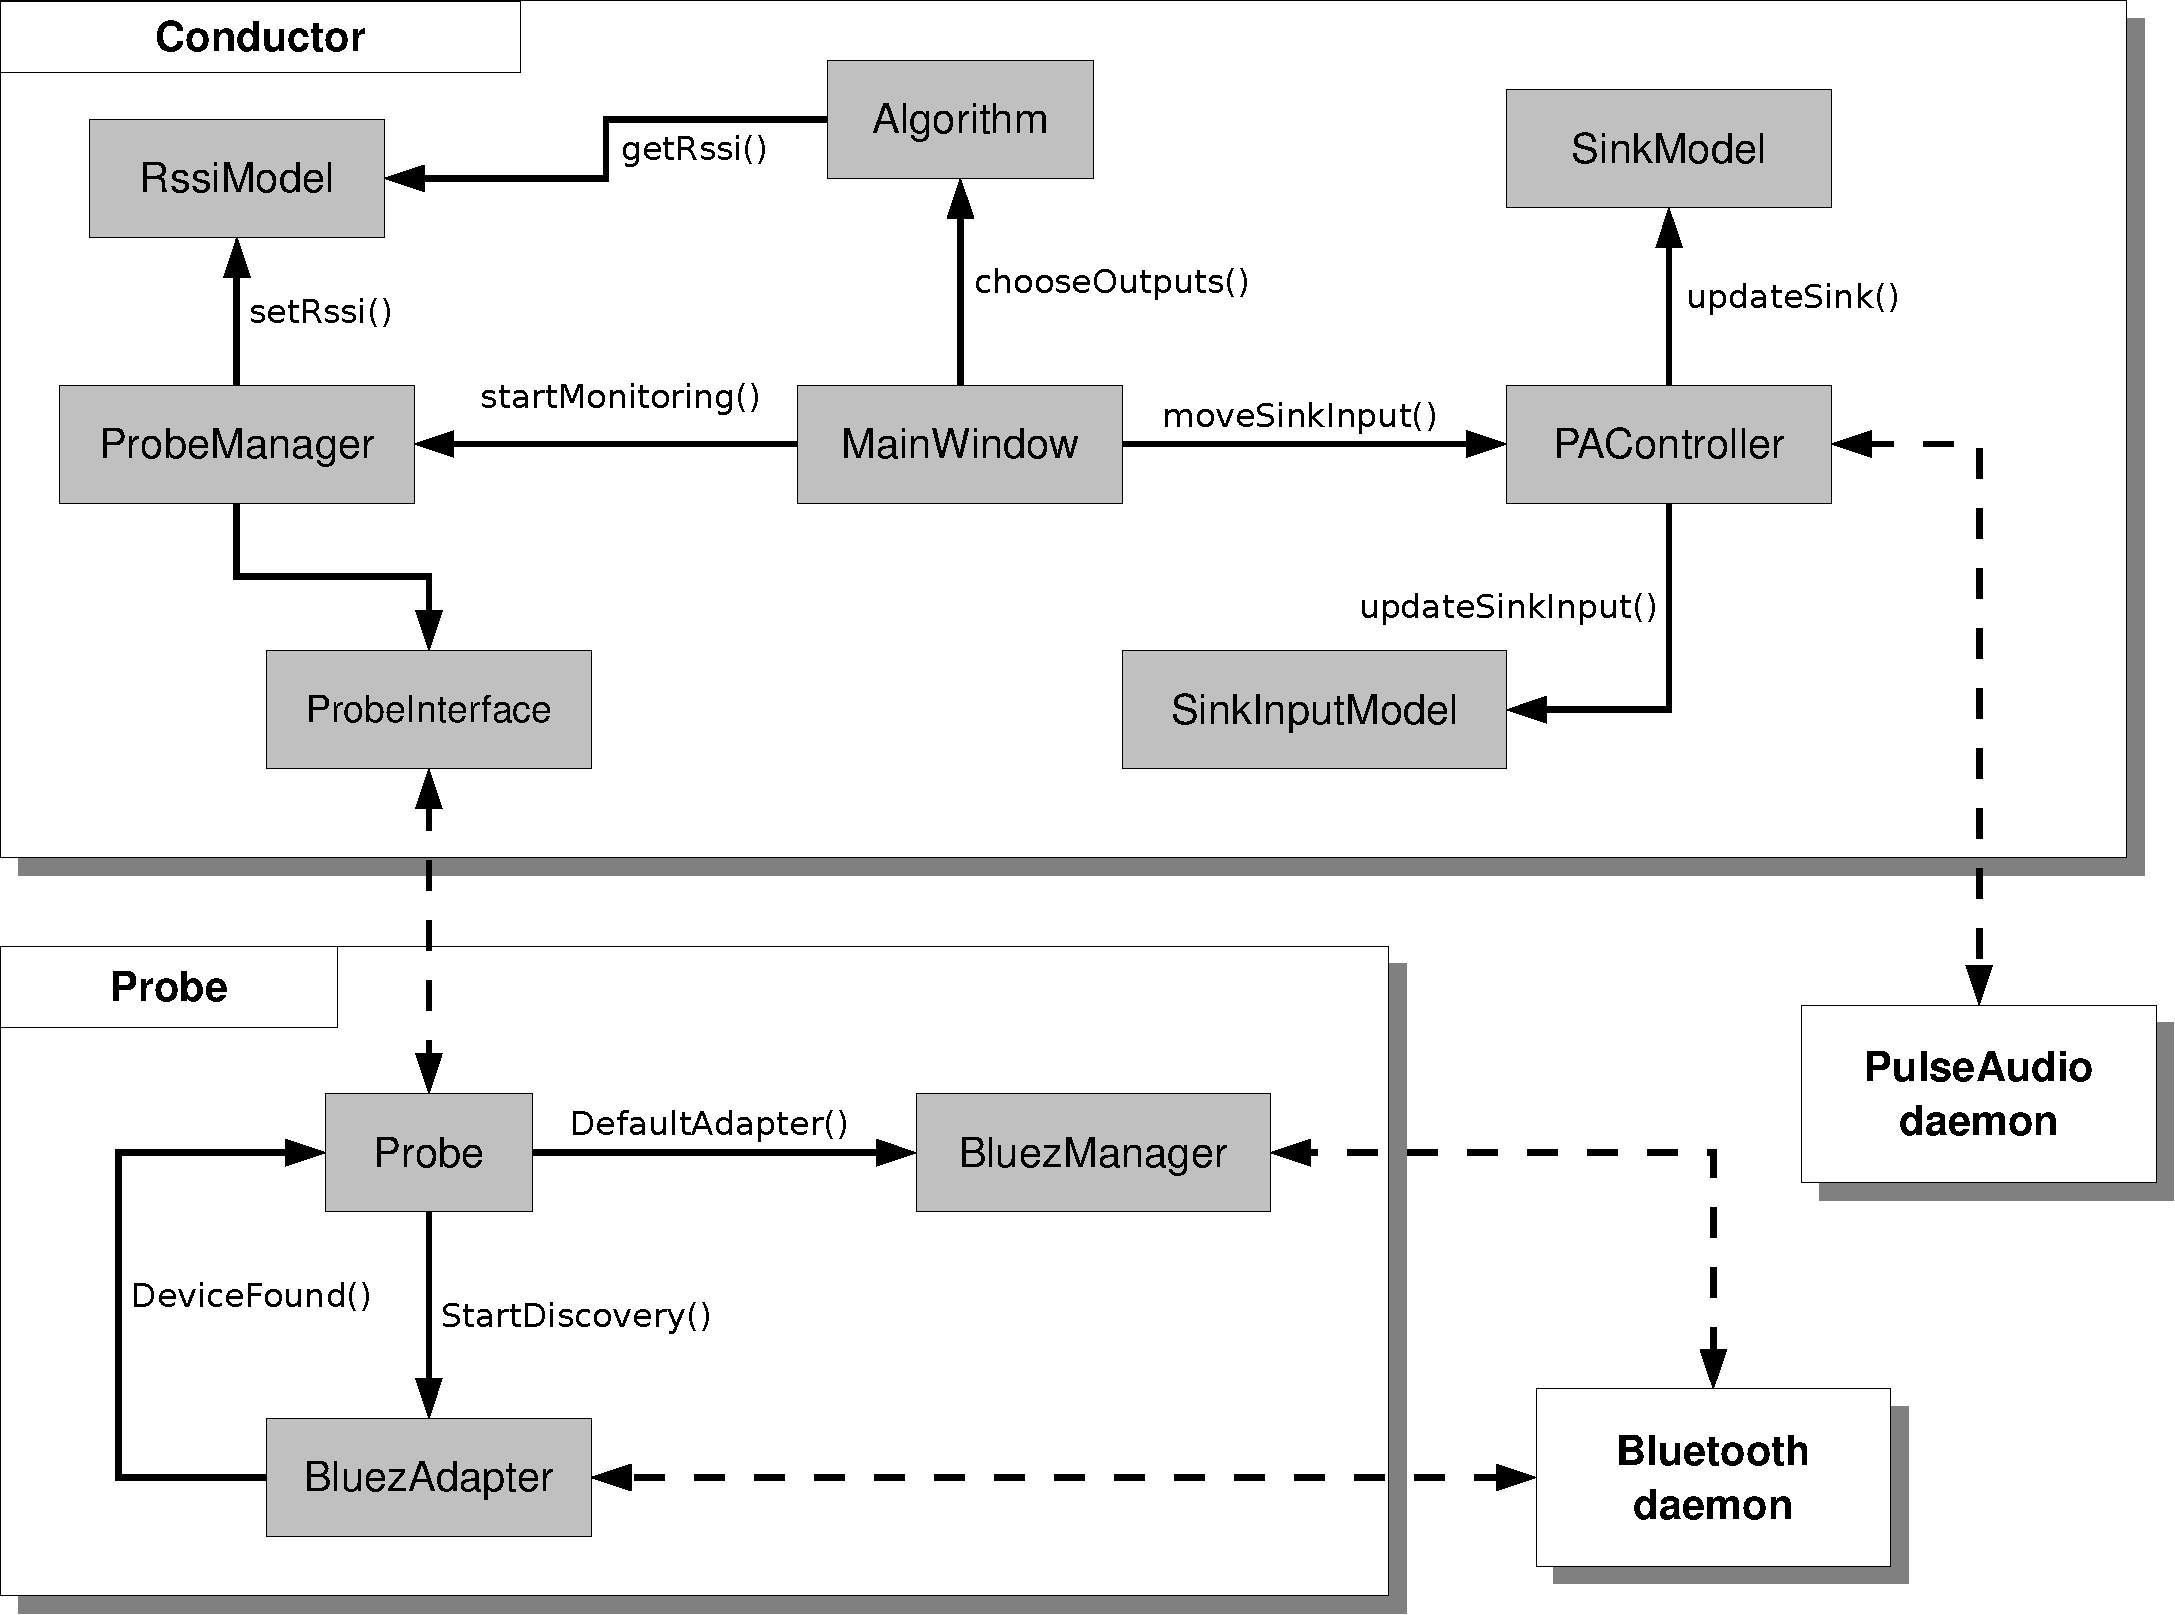
\includegraphics[scale = 0.25]{../Arch}};
    			\onslide<2>
    			\draw[red,ultra thick,rounded corners] (2.6,5.15) ellipse (8mm and 2.5mm);
    			\draw[red,ultra thick,rounded corners] (2.45,1.25) ellipse (8mm and 2.5mm);
    			\onslide<3>
    			\draw[red,ultra thick,rounded corners] (1.05,1.35) ellipse (8mm and 2.5mm);
    			\onslide<4>
    			\draw[red,ultra thick,rounded corners] (1.35,5.5) ellipse (8mm and 2.5mm);
    			\onslide<5>
    			\draw[red,ultra thick,rounded corners] (4.1,6.1) ellipse (17mm and 8mm);
    			\onslide<6>
    			\draw[red,ultra thick,rounded corners] (5.55,5.1) ellipse (8mm and 2.5mm);
    			\onslide<7>
		\end{tikzpicture}
		\end{center}
	\end{frame}
	
	\begin{frame}
		\frametitle{Hardware requirements}
		Here we list the hardware requirements.
		\pause
		\begin{itemize}
		\item \textbf{Smartphone} identifies the room in which the person is.
		\item \textbf{Central server} hosts the main control application.
		\end{itemize}
		\pause
		And for each rooms:
		\begin{itemize}
		\item a \textbf{speaker} that lets out sound when selected to reproduce audio;
		\item a \textbf{Bluetooth adapter} that detects the RSSI value and sends it to the server.
		\end{itemize}
	
	\end{frame}
	
	
	\begin{frame}
		\frametitle{Issues raised during the implementation}
		Here is the list of issues encountered.
		\begin{itemize}
		\pause
		\item Available hardware is unsuitable, it doesn't satisfy the previous requirements.
		\pause
		\item Transferring audio stream throught Pulseaudio is not so reliable (latency, incorrect sampling). Clearly this is not a mature feature. 
		\pause
		\item Pulseaudio operations are asyncronous, so it's difficult to manage and control them.
		\end{itemize}
	\end{frame}
	
%______________________%

\section{Future work and possible extensions}

	
	\begin{frame}
		\frametitle{Future extensions}
		\begin{itemize}
		\item \textbf{Testbed improvement:} the prototype has been tested in a simulated environment disregarding many real conditions. It can be advisable to perform a more through testing session in a real-world scenario. 
		\pause
		\item \textbf{Multiple devices managing:} it could be interesting to consider a context with more than one device to locate. This could entail problems with devices interaction that have to be considered.
		\pause
		\item \textbf{Control's user addition:} a mobile application that allows to the user to control the audiostream (adjust volume, stop/pause, next/previous, \ldots) could increase user interaction.
		\end{itemize}
	\end{frame}
	
%______________________%

\section{Conclusions}
	\begin{frame}
		\frametitle{Final considerations}
		\begin{itemize}
		\item Bluetooth technology: low energy, but variability in managing RSSI values.
		\pause  
		\item Pulseaudio: the audio stream transferring is not reliable.
		\pause
		\item Prototype: it's a good starting point for future improvements and extensions.
		\end{itemize}
	\end{frame}


	\begin{frame}
		\frametitle{References}
		\begin{itemize}
		\item\textbf{PulseAudio Sound Server} \\ \url{http://www.pulseaudio.org/}
		\item\textbf{PulseAudio API documentation} \\ \url{http://0pointer.de/lennart/projects/pulseaudio/doxygen/}
		\item\textbf{BlueZ: the official Linux Bluetooth protocol stack}\\ \url{http://www.bluez.org/}
		\end{itemize}
		
	\end{frame}

\end{document}
